\documentclass{article}

%Package Part
\usepackage{relsize,setspace}  % used by latex(describe( ))
\usepackage{url}               % used in bibliography
\usepackage[superscript,nomove]{cite} % use if \cite is used and superscripts wanted
% Remove nomove if you want superscripts after punctuation in citations
\usepackage{lscape}            % for landscape mode tables
\textwidth 6.75in              % set dimensions before fancyhdr 
\textheight 9.25in
\topmargin -.875in
\oddsidemargin -.125in
\evensidemargin -.125in
\usepackage{fancyhdr}          % this and next line are for fancy headers/footers
\pagestyle{fancy}
\newcommand{\bc}{\begin{center}}  % abbreviate
\newcommand{\ec}{\end{center}}

\usepackage{Sweave}
\begin{document}

\Sconcordance{concordance:khb_report.tex:khb_report.Rnw:%
1 18 1 1 0 14 1 1 27 4 1 1 2 26 0 1 1 13 0 1 1 14 0 1 1 26 0 1 2 2 1 1 %
6 1 2 5 1 1 2 1 3 1 2 4 1 1 2 1 3 1 2 2 1 1 2 1 3 1 2 4 1 1 2 1 3 1 2 3 %
1 1 2 1 3 1 2 2 1 1 2 1 3 1 2 4 1 1 2 1 3 1 2 3 1 1 2 1 3 1 2 2 1 1 2 1 %
3 1 2 2 1}


%\SweaveOpts{width=6, height=4}


\title{Performance Analysis}
\author{}
\date{}

\setkeys{Gin}{width=1\textwidth}
\maketitle
%\tableofcontents


\section{Overview}
This documents go through performance of Simulation. Simulation period is from 2004-11-30 to 2013-03-27. Data sources are WiseFN and Bloomberg.

\subsection{Tables}
% latex table generated in R 2.15.2 by xtable 1.7-1 package
% Fri May 03 16:21:52 2013
\begin{table}[ht]
\centering
\caption{Calendar Returns} 
\begin{tabular}{rrrrrrrrrrr}
  \hline
 & 2004 & 2005 & 2006 & 2007 & 2008 & 2009 & 2010 & 2011 & 2012 & 2013 \\ 
  \hline
1 &  & 2.40 & 5.10 & -3.40 & -2.30 & 7.00 & 1.30 & 1.30 & -0.10 & -0.20 \\ 
  2 &  & 0.00 & -2.90 & -0.20 & 3.70 & -6.00 & 0.40 & 0.00 & 3.50 & 0.80 \\ 
  3 &  & 0.00 & 3.00 & -0.20 & 1.30 & 6.60 & 6.20 & 5.10 & 0.00 & -2.70 \\ 
  4 &  & -4.30 & 5.30 & 3.20 & 7.00 & 8.90 & 2.60 & 1.20 & -1.50 &  \\ 
  5 &  & 4.40 & 0.00 & 0.40 & 1.30 & 0.00 & 0.00 & 0.00 & 0.00 &  \\ 
  6 &  & 3.10 & 6.80 & -0.70 & 0.00 & 0.00 & 2.40 & -0.50 & 1.40 &  \\ 
  7 &  & 0.00 & -0.60 & 8.90 & 0.30 & 11.90 & 0.80 & 2.70 & -1.30 &  \\ 
  8 &  & 0.00 & 2.30 & 4.80 & 0.90 & 1.70 & 1.70 & 0.00 & 2.40 &  \\ 
  9 &  & 3.60 & -0.10 & 3.80 & 6.00 & -1.10 & 3.40 & -1.50 & 0.30 &  \\ 
  10 &  & 0.00 & 3.50 & 1.40 & 0.00 & -3.40 & -0.40 & 7.70 & 0.00 &  \\ 
  11 & -1.00 & 5.50 & 0.00 & 0.00 & 2.20 & -2.80 & 0.00 & -2.50 & 0.00 &  \\ 
  12 & -0.90 & 1.40 & 2.40 & -0.10 & -3.40 & 8.10 & 5.80 & -3.00 & 3.80 &  \\ 
  LongOnly & -1.90 & 16.80 & 27.40 & 18.80 & 17.90 & 33.30 & 26.90 & 10.30 & 8.60 & -2.20 \\ 
  Asset\_prc & 1.60 & 49.40 & 3.80 & 27.90 & -43.00 & 46.70 & 20.70 & -14.10 & 9.70 & -0.90 \\ 
  LongShort & -5.50 & -6.50 & 36.80 & 15.70 & 74.00 & -1.10 & 29.00 & 32.60 & 6.30 & -5.40 \\ 
  ShortOnly & -3.60 & -20.60 & 8.00 & -2.30 & 47.60 & -26.50 & 1.60 & 20.40 & -2.00 & -3.20 \\ 
   \hline
\end{tabular}
\end{table}% latex table generated in R 2.15.2 by xtable 1.7-1 package
% Fri May 03 16:21:52 2013
\begin{table}[ht]
\centering
\caption{Annualized Returns} 
\begin{tabular}{rrrrr}
  \hline
 & LongOnly & Asset\_prc & LongShort & ShortOnly \\ 
  \hline
Annualized Return & 0.18 & 0.08 & 0.18 & 0.00 \\ 
  Annualized Std Dev & 0.11 & 0.21 & 0.18 & 0.14 \\ 
  Annualized Sharpe (Rf=0\%) & 1.65 & 0.37 & 1.04 & 0.01 \\ 
   \hline
\end{tabular}
\end{table}% latex table generated in R 2.15.2 by xtable 1.7-1 package
% Fri May 03 16:21:52 2013
\begin{table}[ht]
\centering
\caption{Returns} 
\begin{tabular}{rrrrr}
  \hline
 & LongOnly & Asset\_prc & LongShort & ShortOnly \\ 
  \hline
Last 12 month return & 2.88 & -1.79 & 2.55 & -0.33 \\ 
  Last 36 month return & 33.05 & 16.70 & 46.59 & 13.54 \\ 
  Last 60 month return & 86.19 & 18.49 & 106.35 & 20.16 \\ 
  Last 101 month return & 145.90 & 83.69 & 155.85 & 9.95 \\ 
   \hline
\end{tabular}
\end{table}% latex table generated in R 2.15.2 by xtable 1.7-1 package
% Fri May 03 16:21:52 2013
\begin{table}[ht]
\centering
\caption{Statistics} 
\begin{tabular}{rrrrr}
  \hline
 & LongOnly & Asset\_prc & LongShort & ShortOnly \\ 
  \hline
Observations & 101.00 & 101.00 & 101.00 & 101.00 \\ 
  NAs & 0.00 & 0.00 & 0.00 & 0.00 \\ 
  Minimum & -0.06 & -0.24 & -0.07 & -0.07 \\ 
  Quartile 1 & -0.00 & -0.02 & -0.02 & -0.02 \\ 
  Median & 0.00 & 0.01 & 0.01 & 0.00 \\ 
  Arithmetic Mean & 0.01 & 0.01 & 0.02 & 0.00 \\ 
  Geometric Mean & 0.01 & 0.01 & 0.01 & 0.00 \\ 
  Quartile 3 & 0.03 & 0.04 & 0.05 & 0.01 \\ 
  Maximum & 0.12 & 0.13 & 0.19 & 0.19 \\ 
  SE Mean & 0.00 & 0.01 & 0.01 & 0.00 \\ 
  LCL Mean (0.95) & 0.01 & -0.00 & 0.01 & -0.01 \\ 
  UCL Mean (0.95) & 0.02 & 0.02 & 0.03 & 0.01 \\ 
  Variance & 0.00 & 0.00 & 0.00 & 0.00 \\ 
  Stdev & 0.03 & 0.06 & 0.05 & 0.04 \\ 
  Skewness & 0.70 & -0.72 & 0.59 & 1.45 \\ 
  Kurtosis & 0.63 & 1.63 & 0.35 & 3.47 \\ 
   \hline
\end{tabular}
\end{table}
\subsection{Distribution}

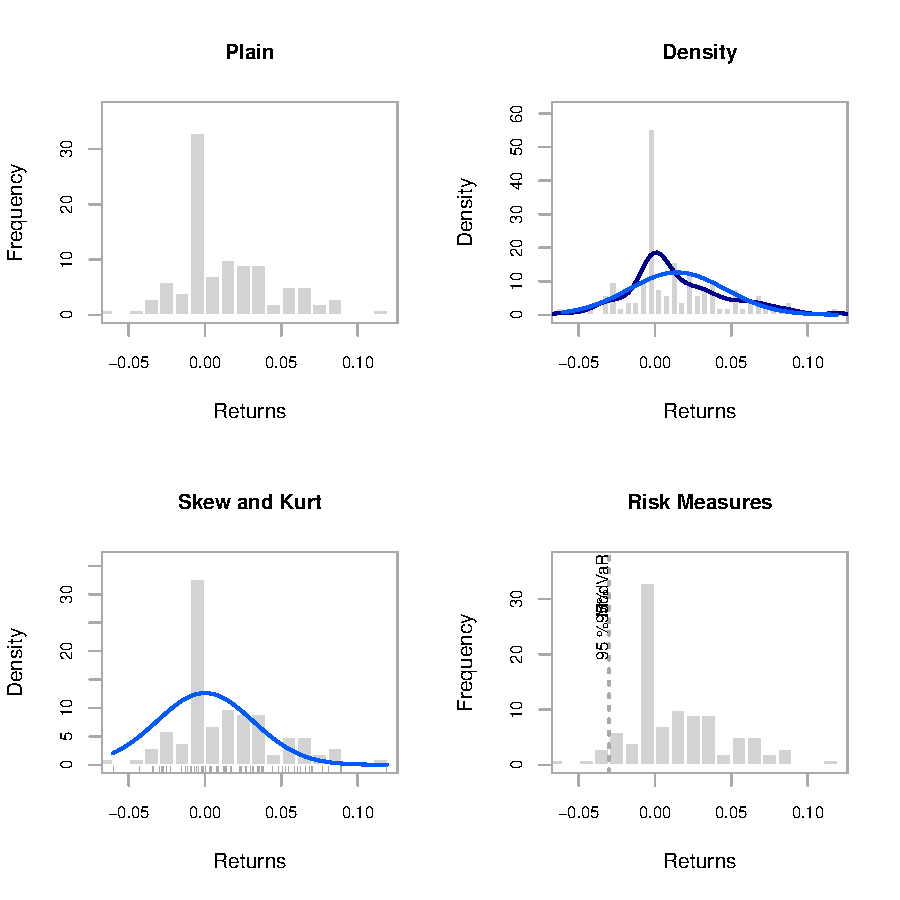
\includegraphics{graphics/plot-003}

\section{All yr Performance}
\setkeys{Gin}{width=0.5\textwidth}
%\begin{landscape}
\subsection{Returns}
\begin{tabular}{cc}
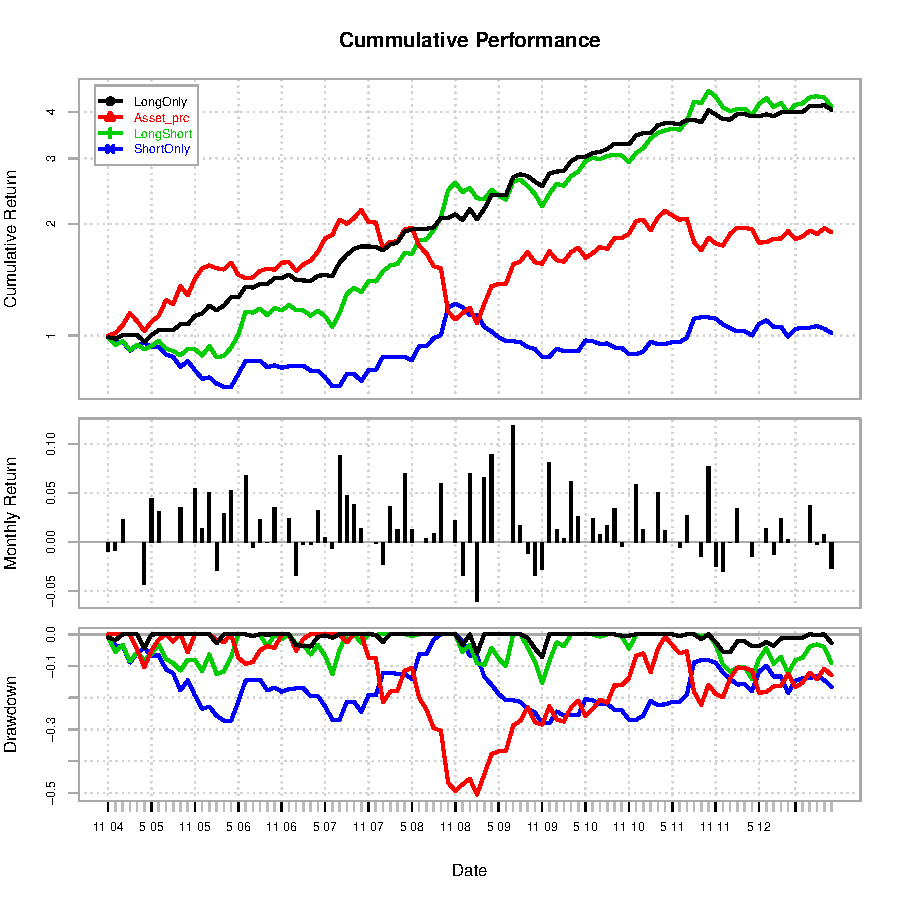
\includegraphics{graphics/plot-004}
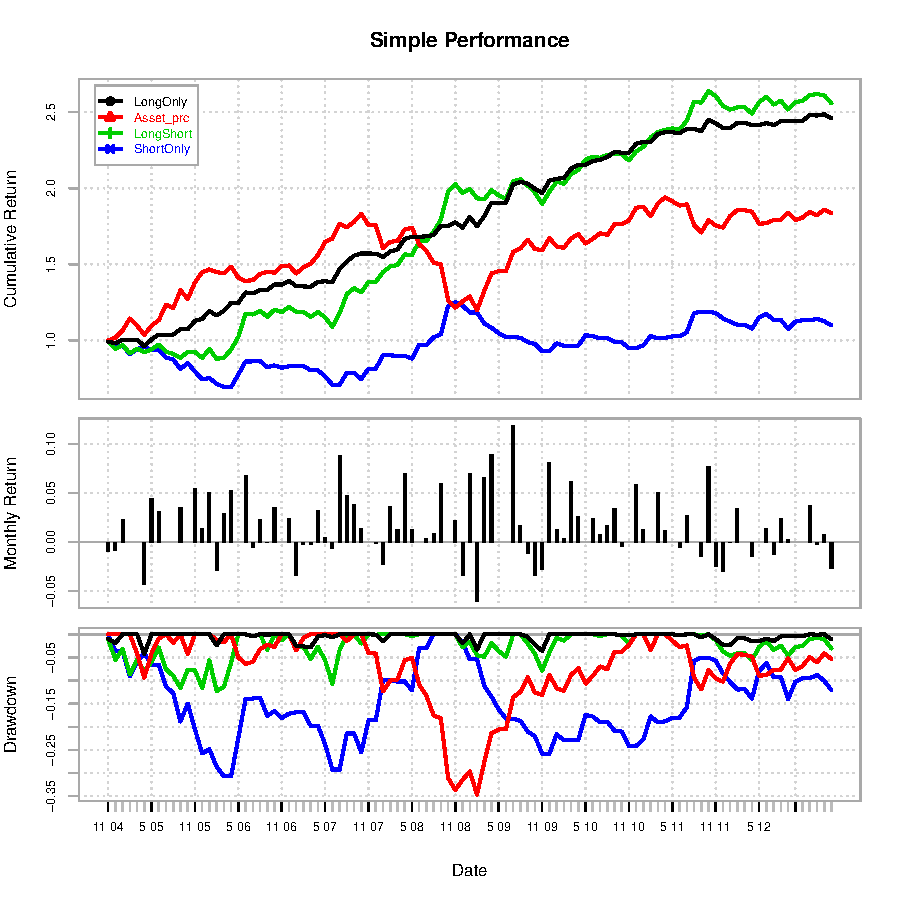
\includegraphics{graphics/plot-005}
\end{tabular}

%\end{landscape}
\subsection{Relative Returns}
\begin{tabular}{cc}
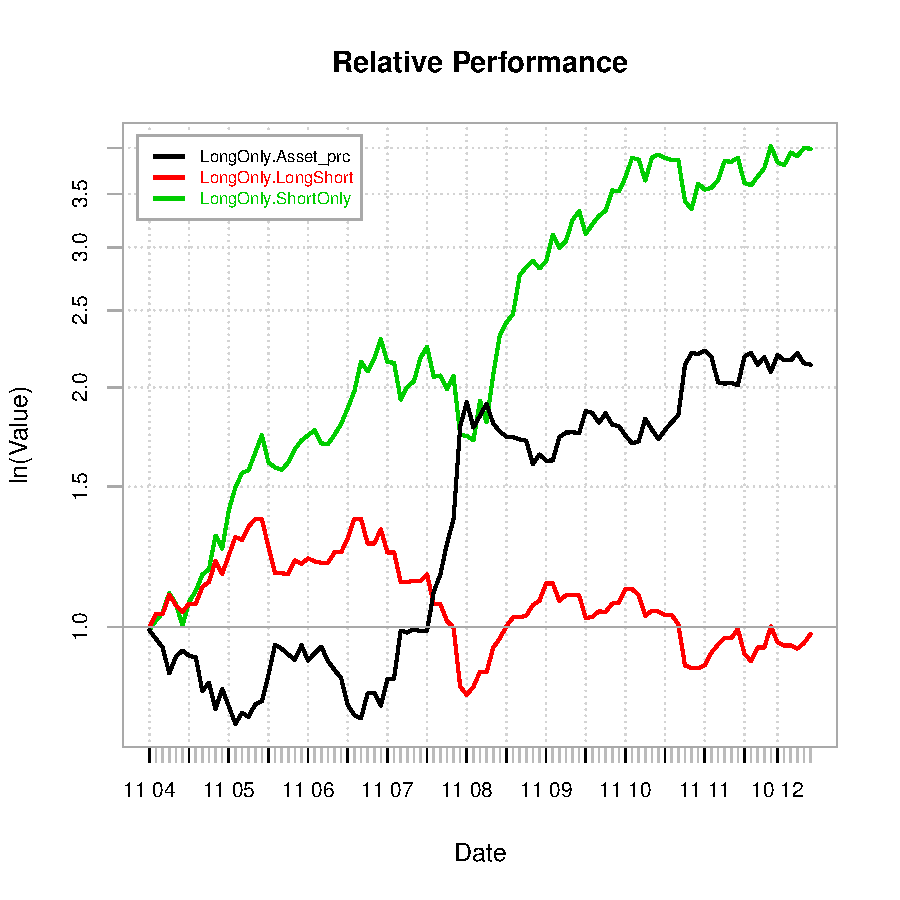
\includegraphics{graphics/plot-006}
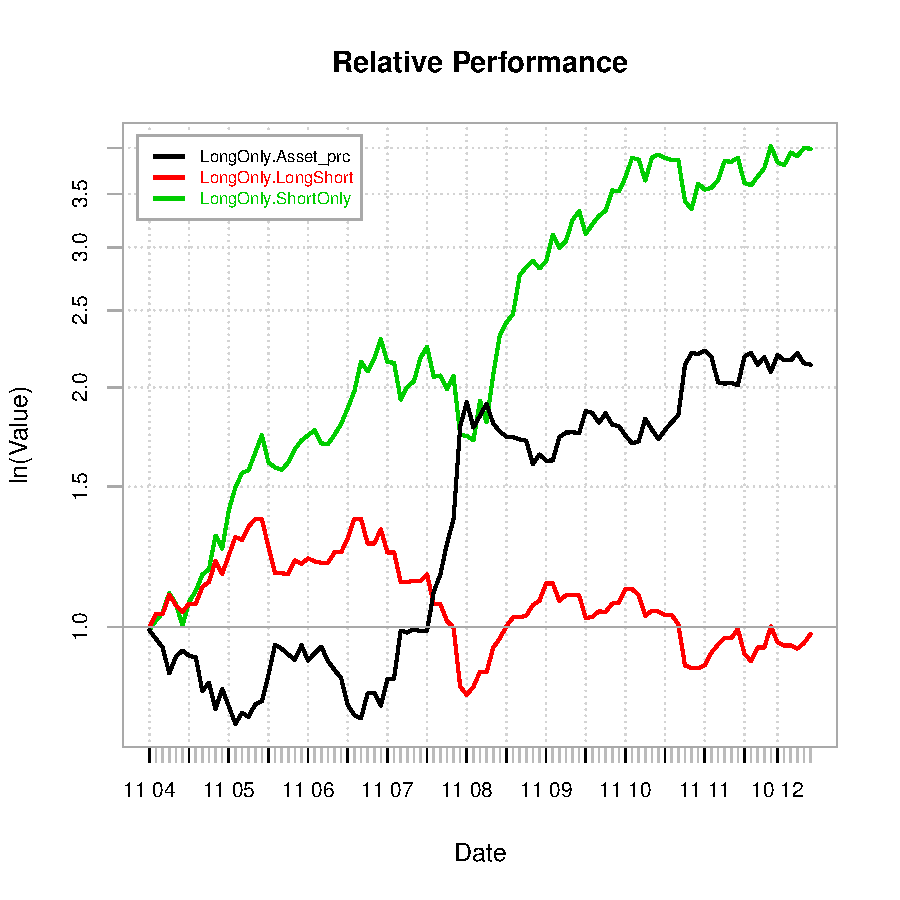
\includegraphics{graphics/plot-007}
\end{tabular}
\subsection{Other Charts}
\begin{tabular}{cc}
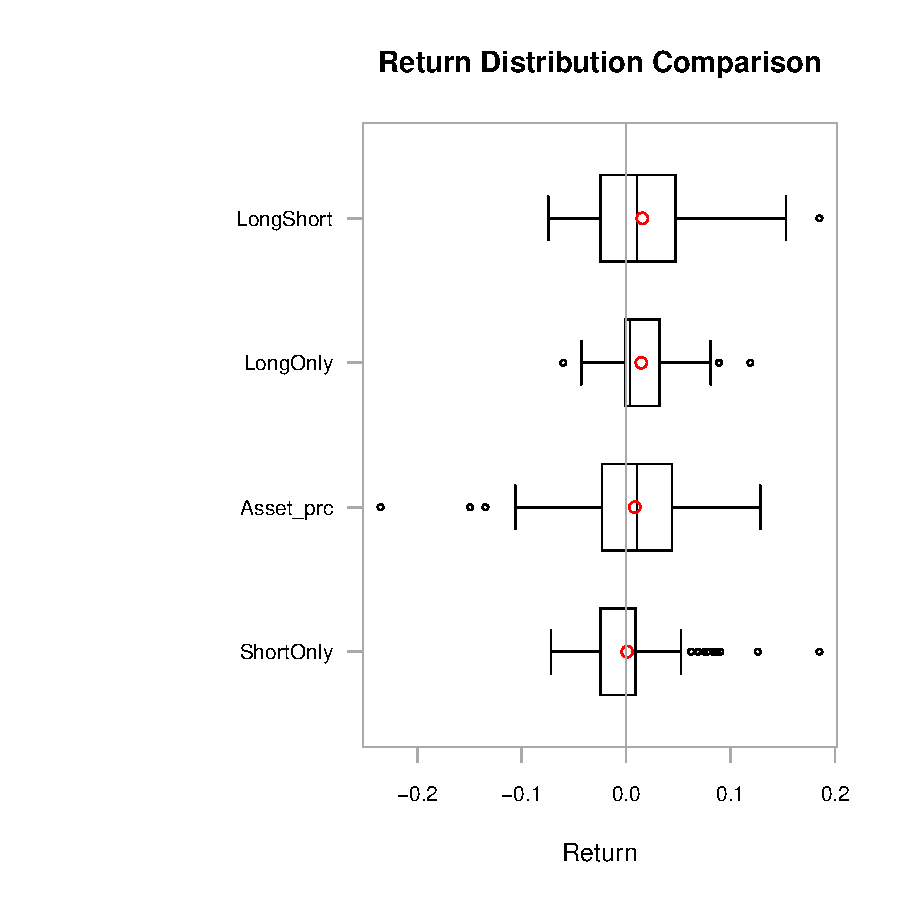
\includegraphics{graphics/plot-008}
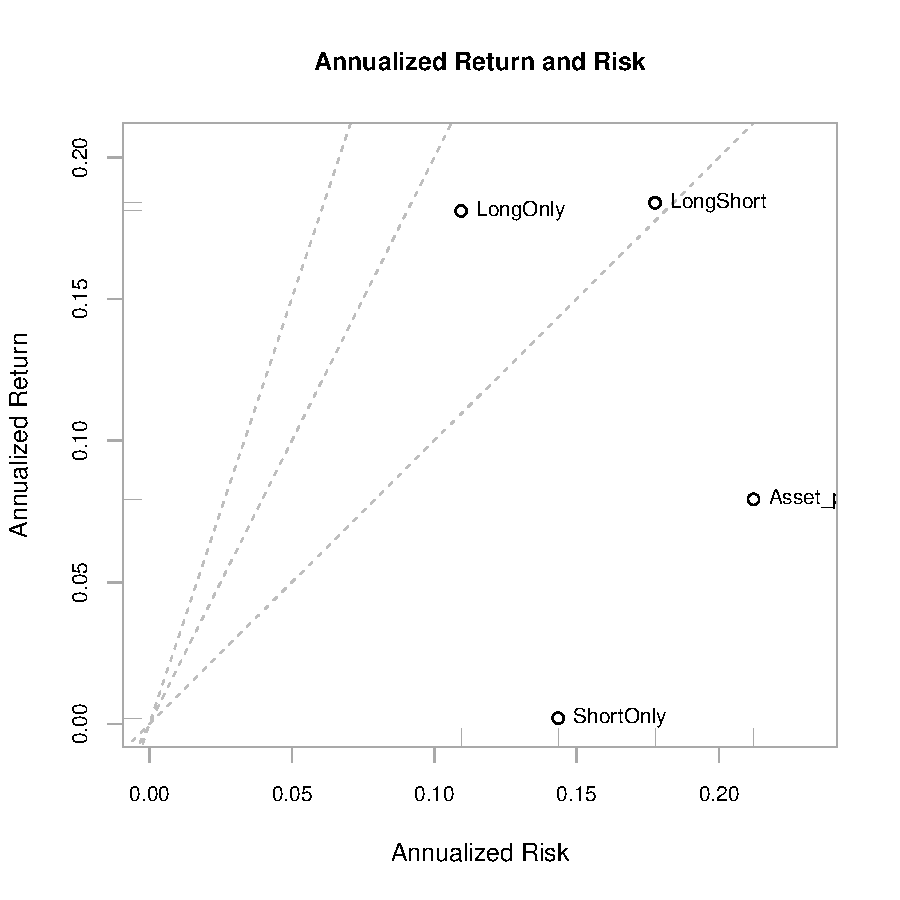
\includegraphics{graphics/plot-009}
\end{tabular}
\section{3yr Performance}
%\begin{landscape}
\subsection{Returns}
\begin{tabular}{cc}
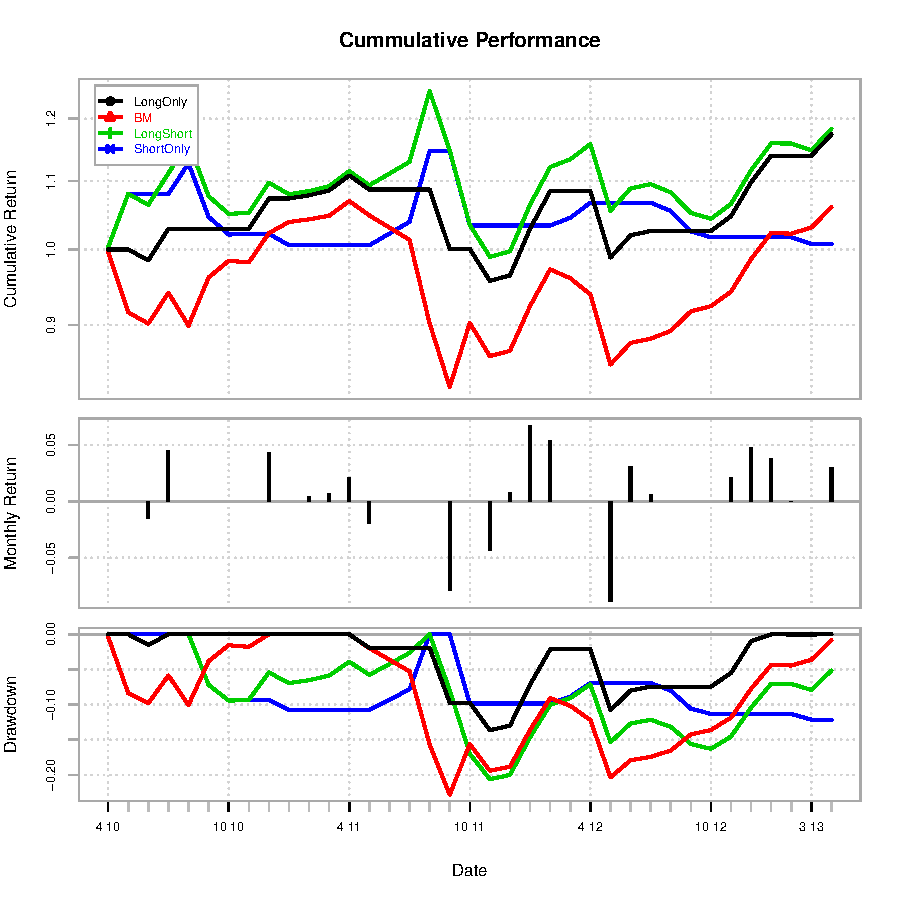
\includegraphics{graphics/plot-010}
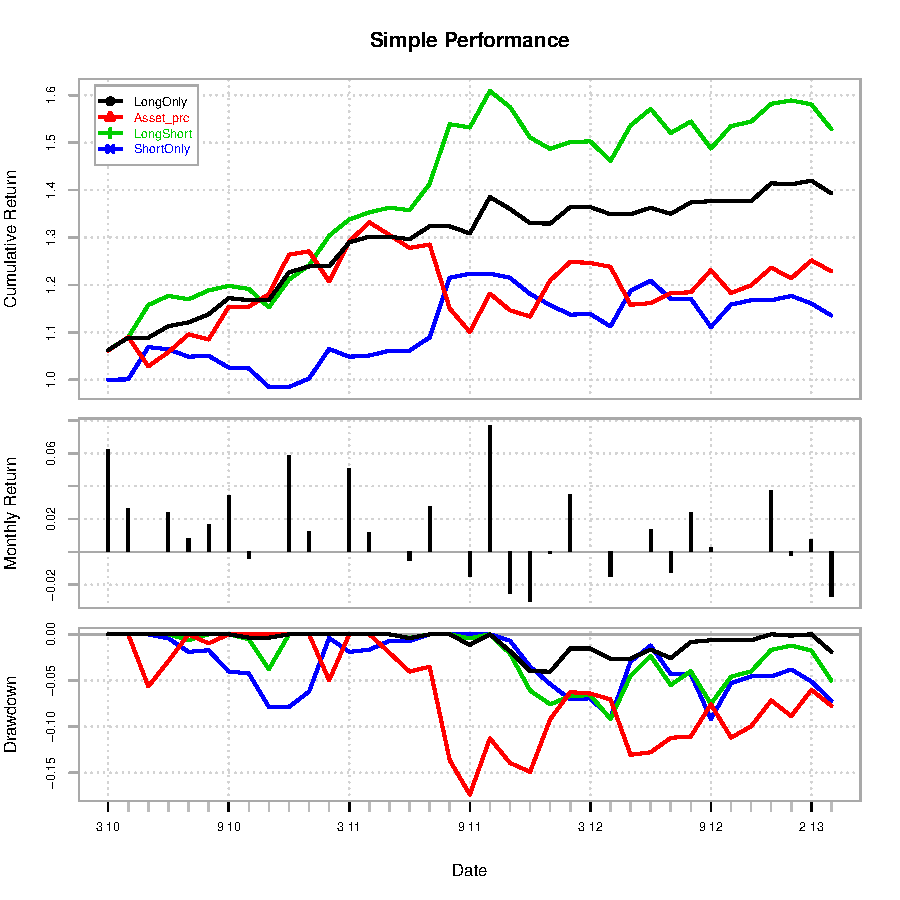
\includegraphics{graphics/plot-011}
\end{tabular}
%\end{landscape}
\subsection{Relative Returns}
\begin{tabular}{cc}
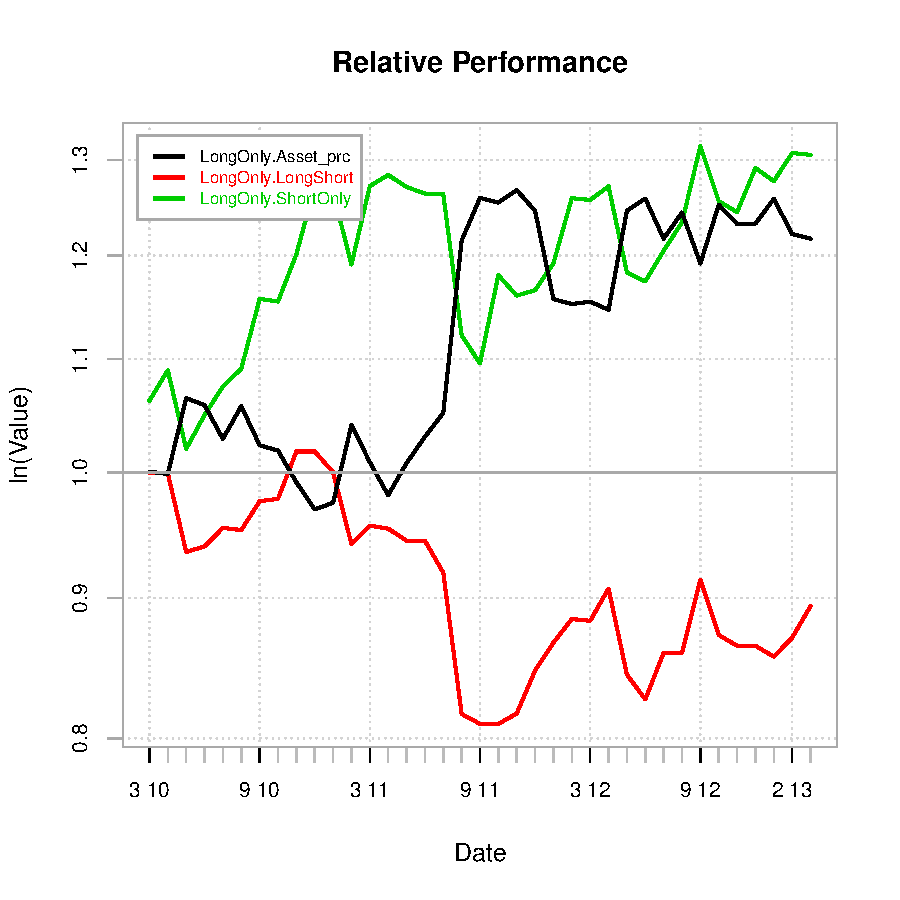
\includegraphics{graphics/plot-012}
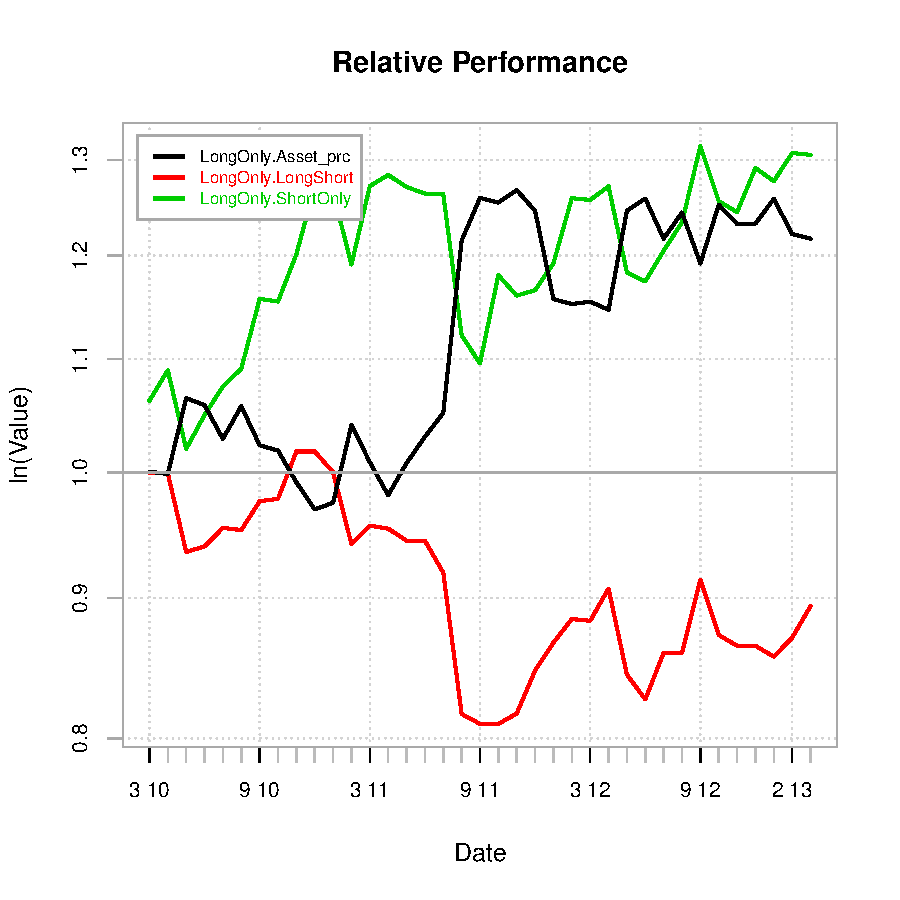
\includegraphics{graphics/plot-013}
\end{tabular}
\subsection{Other Charts}
\begin{tabular}{cc}
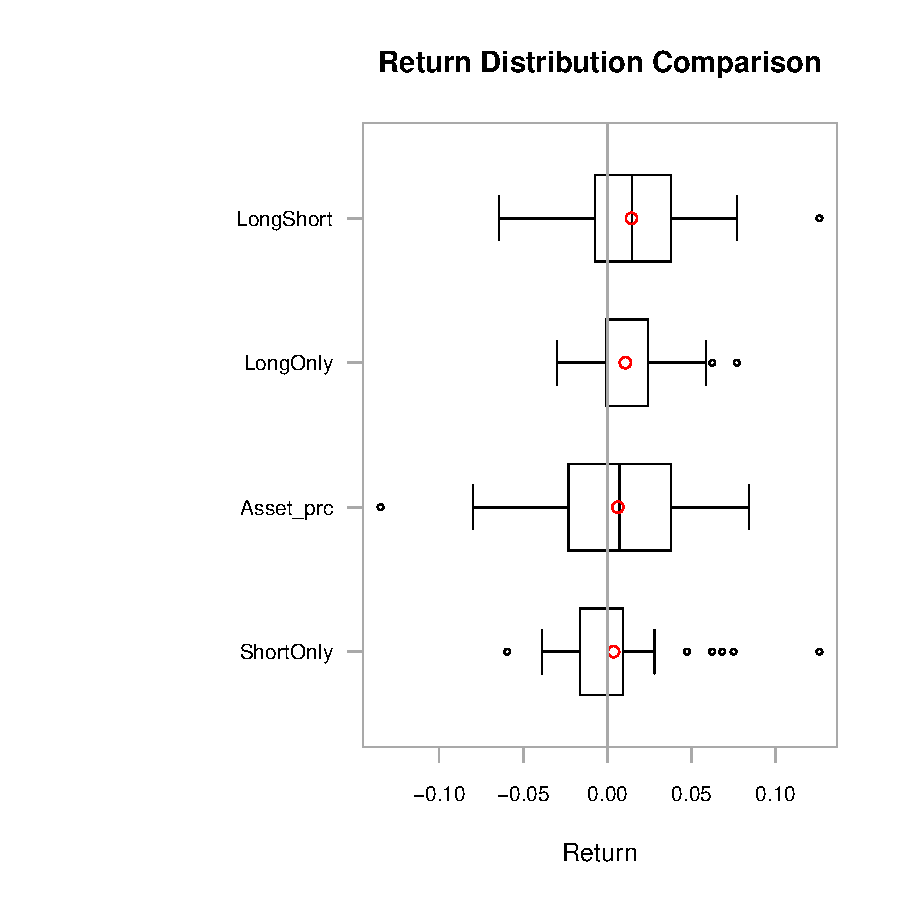
\includegraphics{graphics/plot-014}
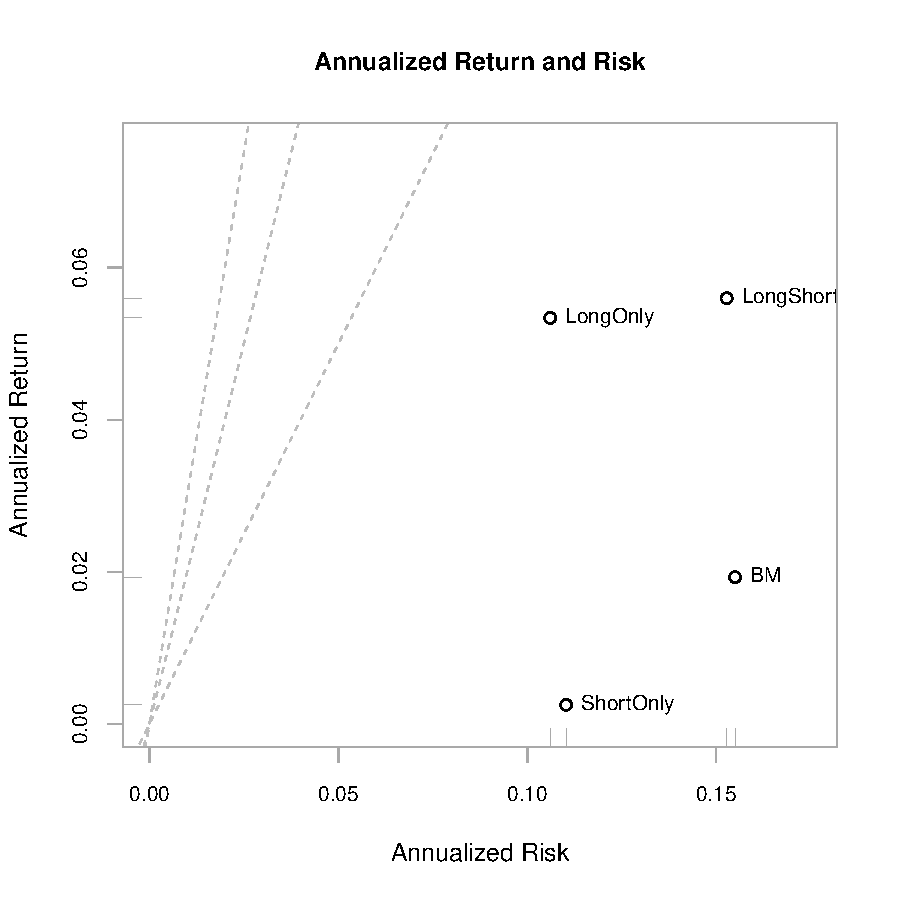
\includegraphics{graphics/plot-015}
\end{tabular}
\section{1yr Performance}
%\begin{landscape}
\subsection{Returns}
\begin{tabular}{cc}
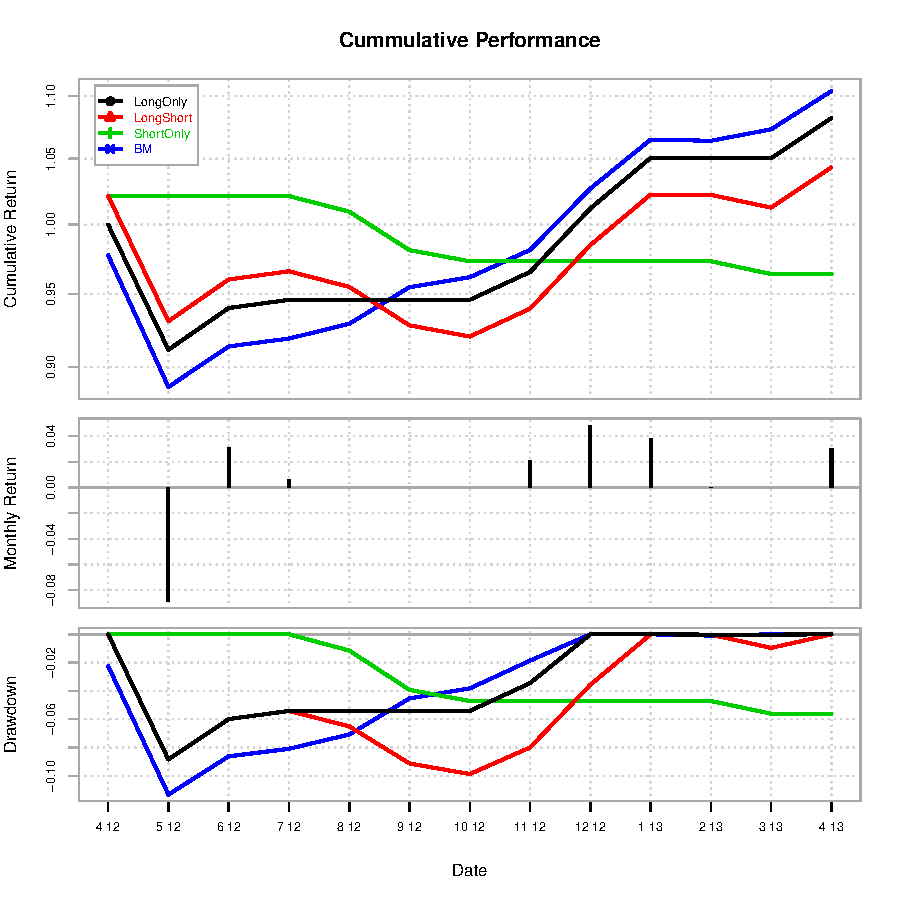
\includegraphics{graphics/plot-016}
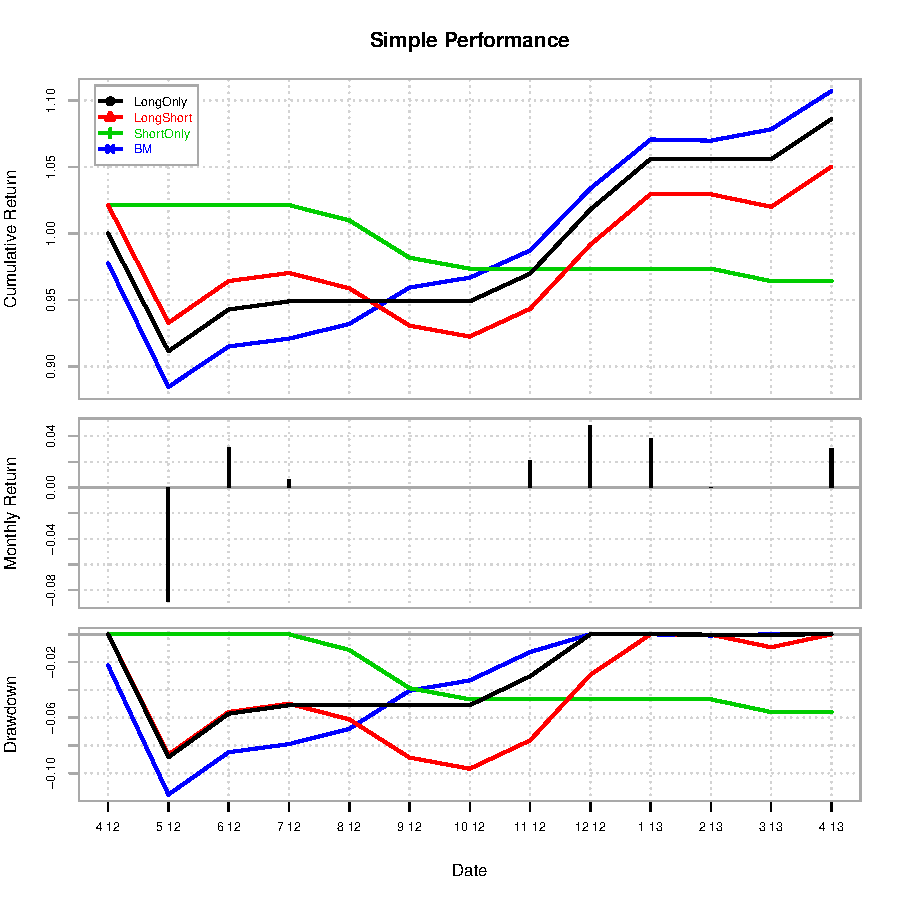
\includegraphics{graphics/plot-017}
\end{tabular}
%\end{landscape}
\subsection{Relative Returns}
\begin{tabular}{cc}
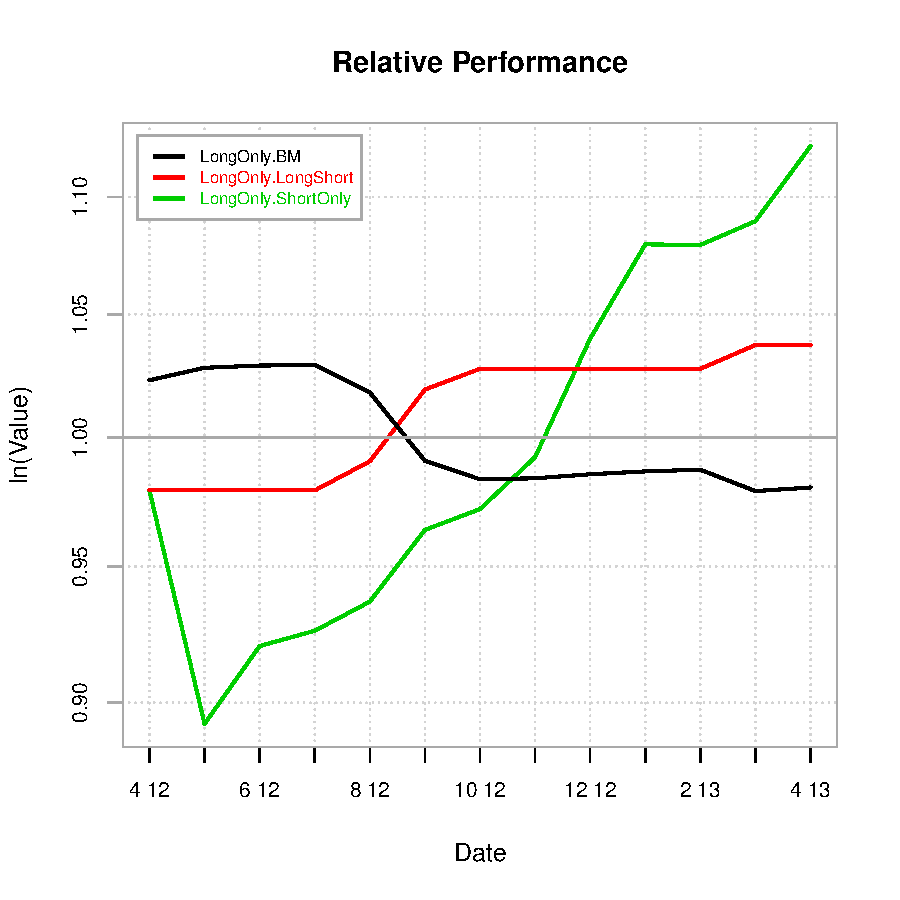
\includegraphics{graphics/plot-018}
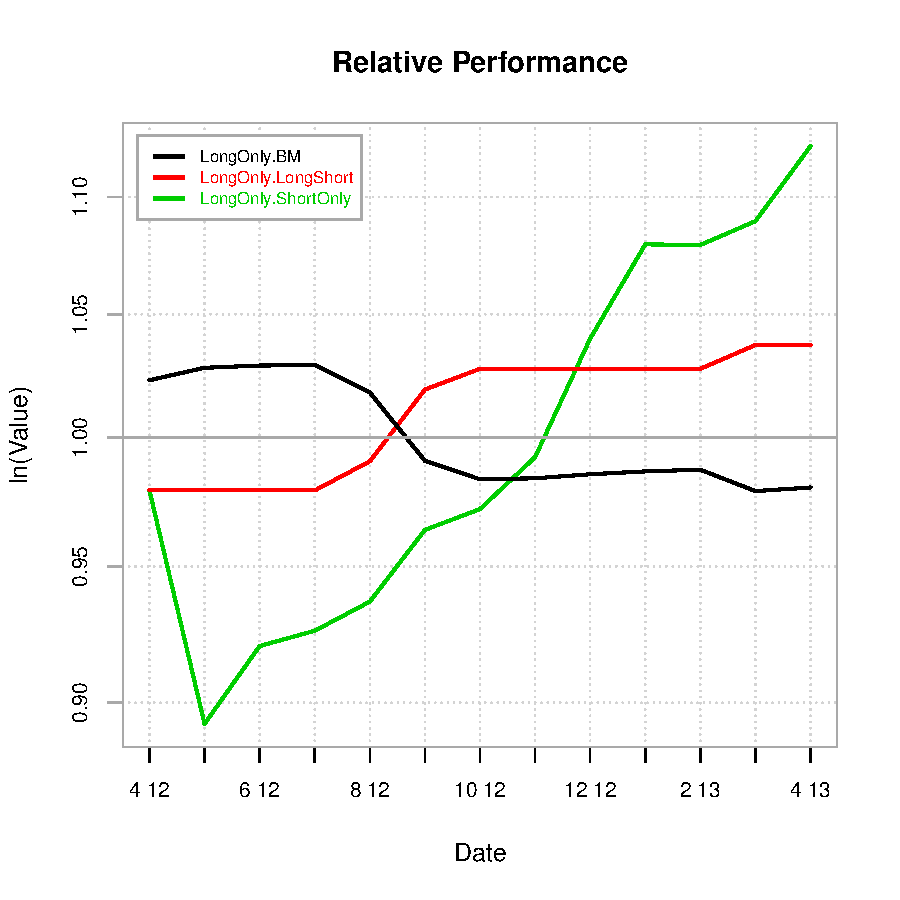
\includegraphics{graphics/plot-019}
\end{tabular}
\subsection{Other Charts}
\begin{tabular}{cc}
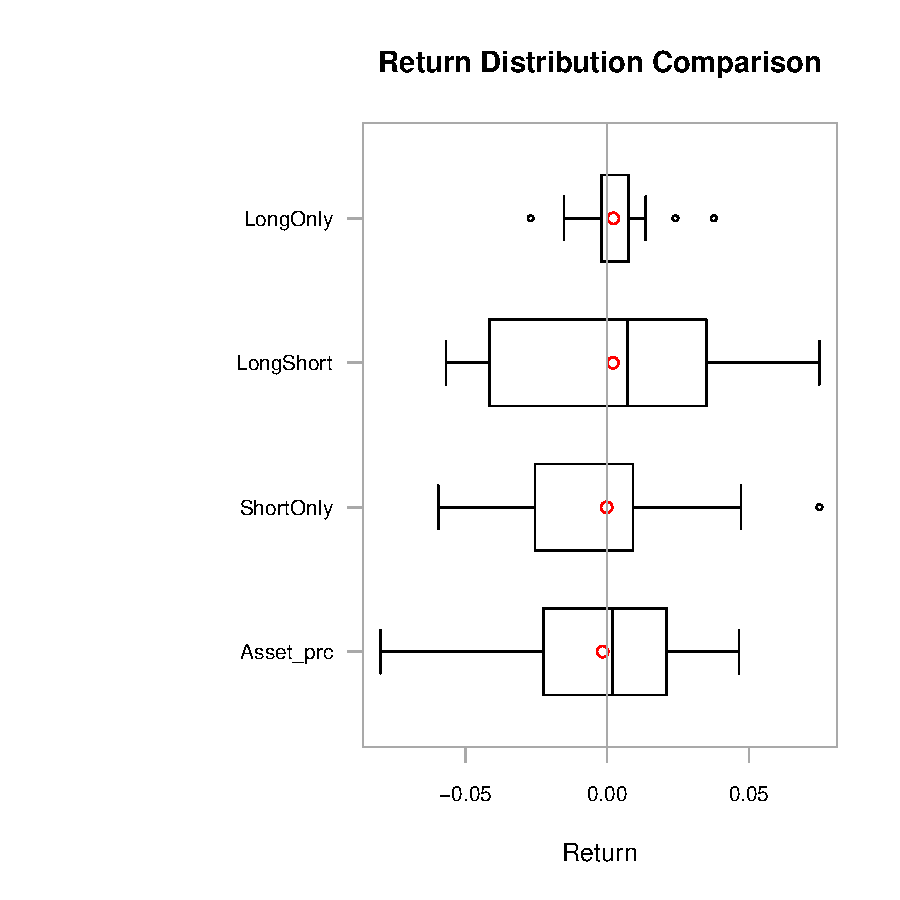
\includegraphics{graphics/plot-020}
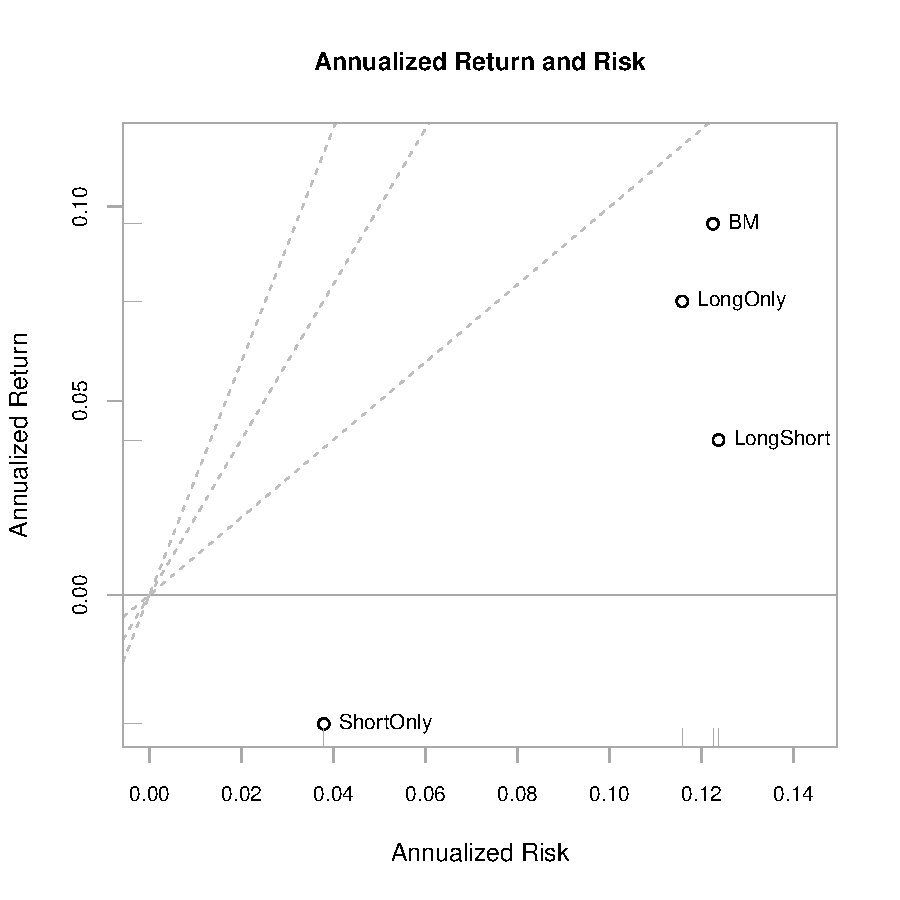
\includegraphics{graphics/plot-021}
\end{tabular}

\end{document}
